\documentclass[conference]{IEEEtran}
% \IEEEoverridecommandlockouts
% The preceding line is only needed to identify funding in the first footnote. If that is unneeded, please comment it out.
% \usepackage{cite}
\usepackage{amsmath,amssymb,amsfonts}
\usepackage{algorithmic}
\usepackage{graphicx}
\usepackage{textcomp}
\usepackage{hyperref}
\usepackage{flushend}

\hypersetup{
    colorlinks=true,
}
\usepackage{xcolor}
% \usepackage[backend=biber,style=numerical,sorting=ynt]{biblatex}
\usepackage[backend=biber,style=numeric,sortcites,sorting=nty,natbib,hyperref]{biblatex}


\addbibresource{sample.bib} %Imports bibliography file

\def\BibTeX{{\rm B\kern-.05em{\sc i\kern-.025em b}\kern-.08em
    T\kern-.1667em\lower.7ex\hbox{E}\kern-.125emX}}
\begin{document}

\title{Runtime Tradeoff in Traffic Monitoring Embedded Systems\\
% {\footnotesize \textsuperscript{*}Note: Sub-titles are not captured in Xplore and
% should not be used}
% \thanks{Identify applicable funding agency here. If none, dont  delete this.}
}


\author{
\IEEEauthorblockN{Pranjal Aggarwal}
\IEEEauthorblockA{\textit{2$^{nd}$ Year UG Student} \\
\textit{Dept. of Computer Science and Engineering} \\
\textit{Indian Institute of Technology, Delhi}\\
New Delhi, India. \\
cs5190443@iitd.ac.in}
\and
\IEEEauthorblockN{Harsh Agrawal}
\IEEEauthorblockA{\textit{2$^{nd}$ Year UG Student} \\
\textit{Dept. of Computer Science and Engineering} \\
\textit{Indian Institute of Technology, Delhi}\\
New Delhi, India. \\
cs1190431@iitd.ac.in}
}



\maketitle
\thispagestyle{plain}
\pagestyle{plain}

\begin{abstract}
In this report, we have analyzed the effect of various computational parameters, and their effect on
accuracy on the computer vision based traffic monitoring systems.
\end{abstract}

% \begin{IEEEkeywords}
% component, formatting, style, styling, insert
% \end{IEEEkeywords}

\section{Introduction}
The recent development of Smart Cities has resulted in an increase in systems capable of monitoring
road traffic for environmental analysis and better traffic management. This requires solutions such as embedded systems,
performing live inference from camera feed of CCTV cameras, deployed across many highways, expressways, and road junctions in the city.
However, these embedded systems are limited on computational capacity and may not have a significant energy source (primarily relying on solar energy).
Also, based on the time of day and day of the year, the varying temperatures add a restriction on how much computational power they can spend without getting overheated.
In this report, we investigate the various computational parameters that can be tweaked, such that the computational load on embedded systems decreases while maintaining
the performance as much as possible. Since we do not have Ground Truth Data,  we create a baseline model, which practically takes the most significant time but is assumed to be the most accurate.
All other models are evaluated against this baseline model. We use Mean Squared Error to analyze the trade-off between the time taken and utility of the model.
The following sections are divided as follows:
In the next section, we will discuss the basic algorithm of the model developed by us to calculate traffic density. This is followed by a section on the metrics used and our
approach to study the effect of runtime and utility. Further in the section, we develop a framework that can assist these systems to make dynamic decisions based on ambient conditions.
In Section 5, we discuss the Trade-Off Analysis, after which we conclude in Section 6.


% \begin{figure}[htbp]
% \centerline{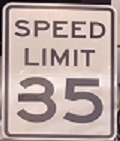
\includegraphics{tesla_speed.png}}
% \caption{By placing a 2 inch black tape on top of sign board researchers tricked a tesla car into speeding to 85mph}
% \label{tesla_speed}
% \end{figure}


\section{Algorithm}
    
We run our algorithm on real footage from a CCTV camera installed at Lajpatnagar junction in New Delhi. \cite{b1}
The camera has a wide range and also doesn't gives a bird's eye view. To solve this, we initially crop each of the frames and correct its perspective to get a bird's eye view. 
For perspective transform, we use OpenCV's \verb|findHomography| and \verb|warpPerspective| algorithm. \cite{b2}
The region to be cropped for a junction is fixed (given the camera orientation) and is taken from the user or is hardcoded.
Then, the background from this image is removed using the \verb|MOG2| algorithm. The algorithm can be trained on an empty photo of the road or using the first few input video frames.
The image is then processed through a series of dilations and erosions, after which we perform binary thresholding. This creates a map of all the vehicles, and helps in calculation of {\bfseries{queue traffic density}}. 
We have deployed two models for \textbf{dynamic density} calculation; one uses Gunner Farneback's algorithm \cite{b4} for solving optical flow equations, while the other is Lucas-Kanade's optical flow algorithm. \cite{b5}
While the former is slower, it yields better results. These algorithms can be switched depending on the computational power available.

\section{Metrics}

Utility error for a given set of test parameters is defined as the mean squared error of densities with respect to the baseline parameters. The error sum is averaged over the entire length of the video. The definition implies greater the error, lesser is the utility and vice versa.
The runtime for a set of parameters is defined as the execution time for processing the video file with the test parameter as input. To ensure results are not varied due to other computer tasks, 
program runs are made on Linux Environment without explicitly running any additional software. For each set of parameters, three runs are performed, and their average is taken to further ensure that external factors do not perturb results.
\section{Methods}

To study the effect of runtime and utility we consider five optimizations:
\begin{itemize}
    \item Frame Sub-Sampling
    \item Image Resolution Reduction
    \item Multi Threading (Spatial)
    \item Multi Threading (Temporal)
    \item Using Sparse Optical Flow
\end{itemize}

In this section effect on utility for each of these is studied independently. The metrics are varied and corresponding 
utility is observed and plotted. Analysis of each of these methods is included in the following subsections itself.

\subsection{Frame Sub-Sampling}

In this method, we only take every $x^{th}$ frame of the video for processing. For the skipped frames, we interpolate the density values from previous frames. We observe that as we increase the number of frames skipped, the time decreases, however the error continuously increases [See Fig~\ref{skf_evt}].
However, we also note that runtime does not change much after skipping more than four frames possibly because loading frames from video starts having a larger relative effect.
Thus we can say for the given model, setting \verb|skip_frames| to 5, is best 
when running on limited performance, as it is able to improve the runtime by a factor of $\approxeq$ 2.5.

\begin{figure}[htbp]
\centerline{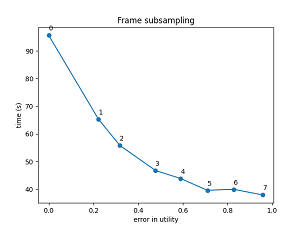
\includegraphics{plots/plot_skip_frames.png}}
\caption{We observe, no suitable advantage is visible on skipping more than 5 frames.}
\label{skf_evt} 
\end{figure}


\subsection{Image Resolution Reduction}

In this method, we reduce the resolution of each frame by a factor. The conversion is done in realtime, and all the processing takes place on this downscaled image.
Unlike frame subsampling, we observe a linearly decreasing graph. However, the difference in error in both of these graphs is significant, with frame subsampling outperforming the current method.

\begin{figure}[htbp]
\centerline{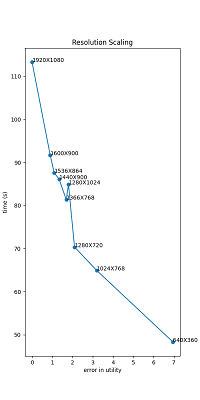
\includegraphics[scale=0.55]{plots/plot_resolution.png}}
\caption{An almost linear increase in utility error with decrease runtime is observed}
\label{res_evt} 
\end{figure}
    

\subsection{Multi-Threading}
Initially, our code was single-threaded, executing statements sequentially, but many independent processes can be executed in parallel to improve the execution time.
We introduced multi-threading in our code to improve the performance by utilizing all cores of a multi-core processor. We have implemented a single producer, multiconsumer threading model using \verb|semaphores|.
A single producer reads the frame from the input video file and places it into a shared buffer. In a multi-threaded environment, several consumer threads are spawned, which wait for the
producer and start processing the frame. \verb|semaphores| are used for thread synchronization and to prevent race conditions among threads for shared memory.

\subsubsection{Spatial} 
We split a frame into segments and assigned each segment to an independent thread. Splitting a frame reduces the matrix size required for each computation and lowers the
thread's average processing time. However, this method also introduces a considerable amount of errors since no thread operates on the borders.
Also, we observe that increasing threads up to 4 has some advantages; however, the runtime also starts growing. One of the reasons is that maintaining a large number of threads
has its own overhead. Moreover, since the sizes of images become small, the runtime advantage of vectorized algorithms is lost.

\begin{figure}[htbp]
\centerline{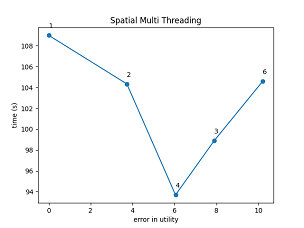
\includegraphics{plots/plot_split_frame.png}}
\caption{We observe to get the least time, 4 threads are needed.}
\label{smt_evt} 
\end{figure}


\subsubsection{Temporal}
We split the work temporally by giving consecutive frames to different threads for processing. The analysis was parameterized by the number of threads used for processing. This method proved quite effective and practically feasible. As the number of threads was increased, the processing time decreased without any significant loss in utility.
However, there was no runtime improvements after more than four parallel threads were used. Because processors have a limit on the number of threads they can use in parallel, and OpenCV algorithms are already heavily vectorized, the saturation is reached early.

\begin{figure}[htbp]
\centerline{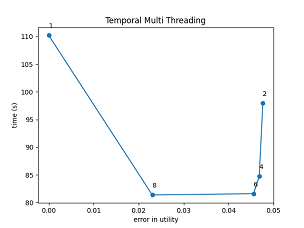
\includegraphics{plots/plot_split_video.png}}
\caption{No sufficient advantage is seen after increasing parallel threads to more than four}
\label{tmt_pvt} 
\end{figure}

\subsection{Sparse Optical Flow}

In this method, we implement the sparse optical flow method for dynamic density calculation instead of the dense optical flow method.
We observe a significant reduction in time taken (roughly 1.8 times). However, the error observed is higher than the other methods.
This behavior is partly due to the sparse method's ability to give zero output when there is actually no movement in the road. This is in contrast to the dense optical flow method,
where there is always some noise. Sparse optical flow yields sufficiently low errors with respect to GroundTruth, and improved runtime. Hence it is an excellent method to keep the computational load in check.

\begin{figure}[htbp]
\centerline{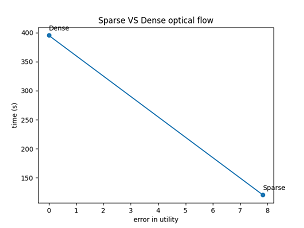
\includegraphics{plots/plot_sparse_optical.png}}
\caption{While decrease in runtime is substantial, we observe error is substantial.}
\label{sof_pvt} 
\end{figure}

\begin{figure}[htbp]
\centerline{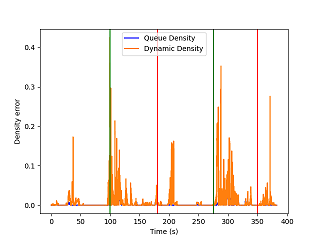
\includegraphics{plots/plot_sparse_dense.png}}
\caption{High Error is observed at points with high dynamic density}
\label{sparse_frame_error} 
\end{figure}

\subsection{Dynamic Tuning}

For embedded systems deployed in production, they must adapt to the environmental conditions. Also, traffic monitoring systems should adjust to the traffic conditions,
i.e, when traffic is low, these embedded systems must switch to low power mode. 
However, it should be noted that facilitating the same is a non-trivial problem. The reason is that different parameters do not correlate with each other in terms of error. Also, no mathematical function exists to map given error to runtime or vice-versa correctly.
To make this dynamic tuning possible, we executed the program on vast combinations of tunable parameters and created a database from the same.
Using a simple c++ function call, based on the error/time constraint, the best metric satisfying the given conditions with the best performance/least error is returned. This best metric is searched from the databse we have created. For example, in a real system, a temperature sensor can send information to tune down performance by $x\%$ and 
the c++ function will return the parameters to be used for the least error.

\begin{figure}[htbp]
\centerline{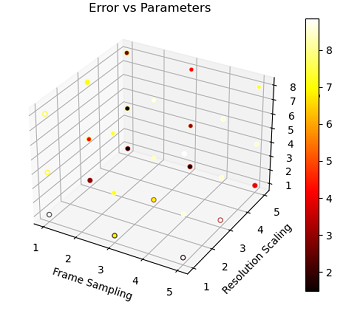
\includegraphics{plots/Error_vs_Params.png}}
\caption{Here z-axis denotes the number of temporal threads used.}
\label{ca_evp} 
\end{figure}
    
\begin{figure}[htbp]
\centerline{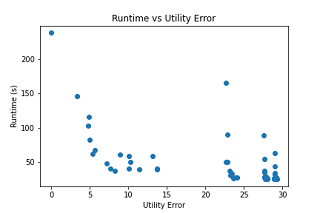
\includegraphics{plots/CompleteAnalysis_rVe.png}}
\caption{The parameters corresponding to bottom left portion of graph are best to use when on a low computational budget}
\label{ca_rve} 
\end{figure}
    
\section{Trade-Off Analysis}

For the various methods, we observe that all have their own advantages. However, we note that frame subsampling can reduce the computational load significantly with the smallest decrease in error.
While temporal multi-threading reduces runtime with no significant error, it is computationally expensive due to multithreading. At the same time, multithreading's full advantage is not 
observed as OpenCV algorithms are already vectorized and optimized, leaving little scope for improvements in user-created threads.
In this report, we also studied the net effect of adjusting various parameters. We observe that parameters are not additive. For example impact of sparse optical flow on lower resolution in terms of time is negligible, however, it induces greater absolute error than on high-res images.
In fact, the best compute-friendly parameters are without sparse optical flow [See Fig.~\ref{ca_rve}].
We also observe that error is maximum during transition zones when either green light turns red or vice-versa. Or in other words, the error is proportional to the queue density, however measuring error relatively, it's roughly the same for the whole video sequence. 
Overall we observe choosing the right set of parameters can decrease computational time significantly (as high as 8-9 times) with minimal error.


\begin{figure}[htbp]
\centerline{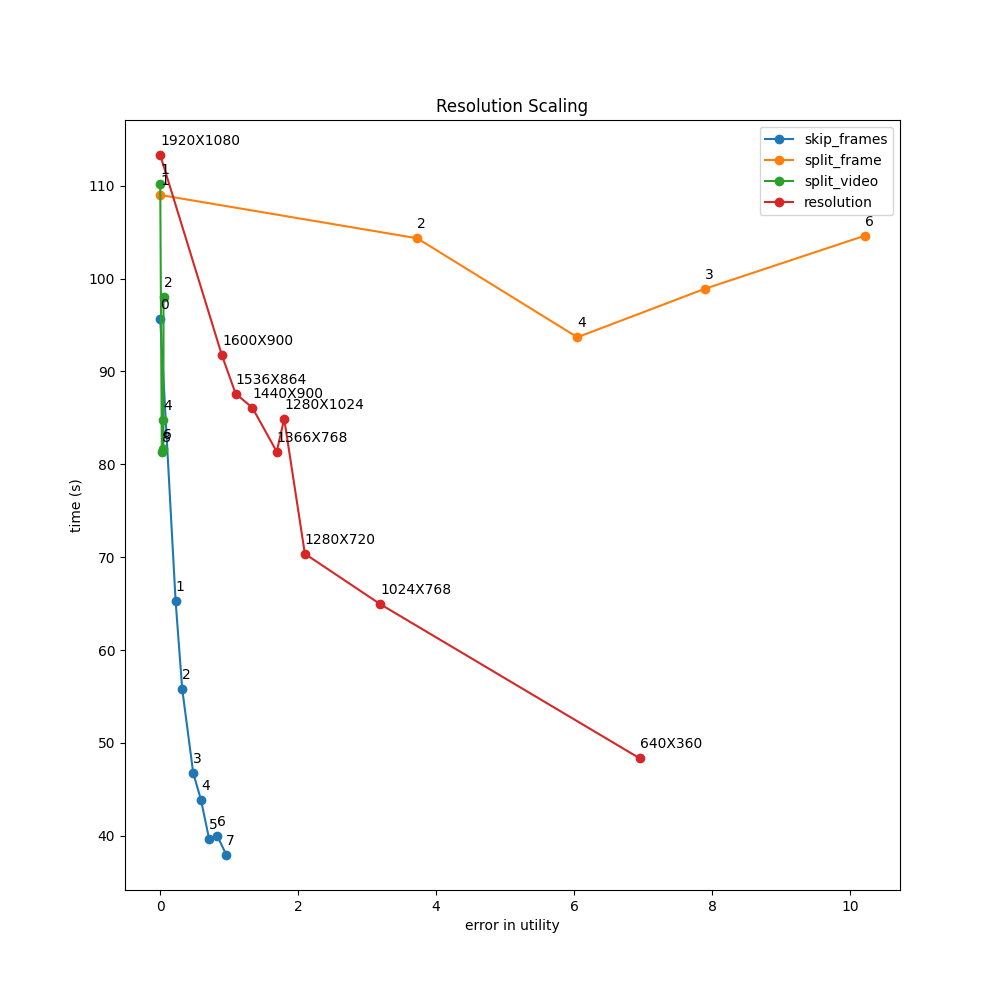
\includegraphics[scale=0.3]{plots/plot_all.png}}
\caption{Skip Frames (blue) ensure maximum improvement in runtime without loss in much error.}
\label{plot_all} 
\end{figure}


\begin{figure}[htbp]
\centerline{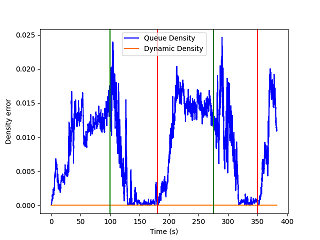
\includegraphics{plots/plot_lowres_error.png}}
\caption{Error is high wherever traffic density is high}
\label{low_res_err} 
\end{figure}
% Graph of all methods combined(eVt) goes here

\section{Conclusion}

In this report, we have studied the effect of tuning parameters on runtime parameters for real-time computer vision based traffic monitoring system.
We see most methods are able to reduce the runtime significantly, with a minor penalty in the accuracy.
We observe that while some methods(frame subsampling) can outperform other methods in almost all cases, to improve the overall runtime, the right combination of multiple methods is needed.
However, if oa single method is used, adjusting frame subsampling to improve runtime is the best choice. Since traffic densities change at a scale of few seconds, decreasing the processing frame rate to 2 FPS will not affect the calculations much.
Overall, we conclude that naive models can be improved substantially by suitable optimizations, making it possible for real-time inference even in embedded systems.



% \section{Inherent Ethical Issues in deep networks}


% \subsection{Racial Discrimination}

% Recent studies have suggested that quite a few computer vision models are biased against blacks.
% In 2020, an experiment got viral on Twitter, which showed that google's vision API would classify a black person's hand with a thermometer gun classified as one carrying guns while a white person would come out clean \cite{b21} \cite{b22}.
% Similarly, In 2015 a google image recognition system would label some black people as gorillas \cite{b20}.
% In 2018 a report indicated that US courts' risk assessment system was biased against blacks and ended up declaring
% blacks being almost twice as likely to re-offend as compared to others. \cite{b15} One reason for making biased decisions against
% blacks in criminal cases could be that despite the low population of blacks in the USA(13.4\%), more than
% 53\% of murder activities were orchestrated by blacks in 2018\footnote{Ofcourse, this has nothing to do with their color, but is possibly due to fact that in general black families have a much lower salary(Median:- \$41,000) as compared to white families(Median:- \$70,000)} \cite{b16}. Since while training models, balancing within a single class is not done, deep networks tend to learn that blacks are more offensive.
% In another study, Ziad Obermeyer et al. showed a widely used algorithm in US hospitals assigned the same risk to a black patient with severe illness than his/her white counterpart \cite{b17}.
% While the above two issues have severe consequences and though did not use computer vision models,
% a model by the name PULSE was release in mid-2020 was capable of upscaling low-resolution human face images by 64 times \cite{b18}.
% While this looks harmless, a controversy broke out in various social media platforms as it would tend to upscale blurred images of black people to that of white people \cite{b19}. This shows that such issues
% may also be present in other critical systems. 
% These facts show that computer vision models and, in general, many ai models are capturing and amplifying general human prejudices.

% \begin{table}[htbp]
% \tiny
% \caption{Serious Crimes by Race in USA(2018)}
% \begin{center}
% \begin{tabular}{|c|c|c|c|c|}
% \hline
% % \textbf{Table}&\multicolumn{3}{|c|}{\textbf{Table Column Head}} \\
% \cline{2-4} 
% \textbf{Serious Offenses} & \textbf{\textit{All Races}}& \textbf{\textit{White}}& \textbf{\textit{Black}} & \textbf{\textit{\% Black Offenders}} \\
% \hline
% Murder & 11,970& 5,280 & 6,380 & 53.30\% \\
% \hline
% Aggravated assault & 395,800 & 245,050 & 133,330 & 33.69\%\\
% \hline
% Vandalism & 179,830 & 121,640 & 51,880 & 28.85\% \\
% \hline
% Arson & 9,390 & 6,670 & 2,350 & 25.03\%\\
% \hline
% Offenses Against Children & 87,480 & 58,950 & 25,190 & 28.80\%\\
% \hline
% Violent crimes & 495,900 & 288,620 & 187,470 & 37.80\%\\
% \hline
% All Serious Crimes & 1,180,370 & 726,210 & 406,600 & 34.45\%\\
% \hline 
% % \multicolumn{5}{l}{dsaknksdn}
% % \multicolumn{5}{l}{Blacks have larger percentage of reported crimes(~35\%) as compared to their population(~13.4\%). }
% % This has got nothing to do with their color but it is mostly due to the fact that while blacks have median salary of \$41,000, whites have median salary of \$70,000.}
% \end{tabular}
% % \caption{Blacks have larger percentage of reported crimes(~35\%) as compared to their population(~13.4\%). 
% % This has got nothing to do with their color but it is mostly} %due to the fact that while blacks have median salary of \$41,000, whites have median salary of \$70,000.}
% \label{tab1}
% \end{center}
% \end{table}

% \subsection{Gender Discrimination}

% Similar to \cite{b22} google's cloud vision API(and in general any other famous vision APIs), Barsan and team showed that on a supposedly randomly chosen sample data,
% the API would classify women wearing a mask as duct tape 28\% times while only 15\% times for men. Also, the accuracy of detecting masks was found to be double that of women \cite{b23}.
% Another study showed that face recognition systems work far better for men than women and, in general, perform too poor for black women \cite{b24}.
% However, one might argue that these systems are harmless, but the fact that these are unpredictable makes the situation worrisome.
% As was the case with a University of Washington study \cite{b25}, which pointed out that women were underrepresented in Google image searches when searched for jobs, including important titles such as CEO.

% \section{Misuse of Computer Vision Systems violating ethics}

% This section will report instances citing various literature on how attackers and malicious actors can use computer vision systems to target individuals and harm them.
% While a large number of fields exist in this section, only 3 of them have been studied in brief.


% \subsection{Espionage and Identity Theft}
% This has been one of the most common and horrible consequences of advancement in computer vision.
% In recent times increased use of social media has revealed that it is possible using computer vision algorithms to extract some of the classification data and metadata from the photos shared by users to make them more identifiable and later result in impersonation \cite{b29}.
% Researchers have also shown that it is possible to extract the biometric signature from egocentric videos of users \cite{b30}. Since it is mostly believed that egocentric videos are good in maintaining privacy, their usage increases with time, thereby putting more people at risk.
% Moreover, with the growth of augmented reality, sharing videos through smart glasses or other devices may lead to a leak of important traits of the user without him/her know that.  
% Another pressing issue in recent times has been that of surveillance. In the name of preventing crime, it is possible that governments across the world, using automated surveillance systems, can track down people of particular identity and then spy on them.
% As reported in the NY Times article \cite{b31} Chinese Government is using cv models for targeting Uighurs Muslims, making it one of the first reported examples of using ethnic profiling software.
% Also, increased surveillance from cameras or smart devices constantly doing inference gives a sense of anxiety and stress, doing psychological harm to people \cite{b43}. For example, this may result in people not attending protests in fear of being caught. 

% \subsection{Misinformation}

% Misinformation is a growing side effect of computer vision. One of its simplest forms is the use of image filters and other image enhancement techniques used in social media.
% There have been a large number of phishing scams because of this. Moreover, a photojournalist can use such techniques to create a bias and prejudice in his articles \cite{b29}.
% With better computer vision techniques, creating fake images and manipulating them has become easier and harder to detect.
% In July 2020, OpenAi released its GPT-3 model\footnote{GPT-3 is a natural language processing model largely known for its text generation capabilities.} in public to be used by researchers and academians. The text generation software was capable of creating fake news given a few starting words, which was indistinguishable from that written by humans \cite{b34}.
% In fact, in one of the articles, The Guardian claimed that one of their whole article was written by it \cite{b33}. Similar to the potential of GPT-3 like models in text generation, deep fakes have potential in fake image/video generation.
% For example, A. Siarohin et al. showed in a research paper that using a driver video, one could animate a source object \cite{b35}. An interesting thing about this is the source object need not be a face but can be any object.
% Moreover, with these codes being publicly available \cite{b36} \cite{b37}, anyone with little technical knowledge can use them to spread misinformation. 
% On 20 July 2020, exactly 51 years after the first Apollo moon landing, MIT released a deepfake video showing the then US President Nixon giving a disaster speech\footnote{The speech was the same as the pre-prepared speech which Richard Nixon would have given in case of any casualty.} (See Fig.~\ref{nixon_generated}), that he had actually never given \cite{b38}. The video has the potential of fooling humans if shown without the disclaimer.
% With such disrupting potentials of spreading misinformation, research in the field of detecting fake information is needed more than ever.
% In fact, a lot of research is already going on in tackling these issues \cite{b51}. The only question is, where will the balance between the two lie.

% \begin{figure}[htbp]
% \centerline{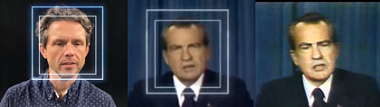
\includegraphics{nixon_combined.png}}
% \caption{Left: Image of Actor used to drive Nixon's fake video. Middle: A single frame from generated Nixon's video. Right: Original Image of the then US President R. Nixon making speech.}
% \label{nixon_generated}
% \end{figure}

% \subsection{Malicious Attacks}

% While this type of attack cannot be directly attributed to computer vision model, its roots still stem from a large number of images and videos we have stored of individuals.
% As argued by Mikael Lauronen \cite{b29} with the growing database in hands of organizations and governments in the form of images/videos of people, gathered either through facial recognition systems or surveillance systems, efforts should be made to make sure that a hacker cannot access this information by accessing a loophole in the system deployed to manage this data \cite{b41}. 

% \section{Conclusion}

% Thus it is evident that growing uses of computer vision models also require a check on its potential misuse. Also, it is time that we make sure that models developed are unbiased in as much capacity as possible.
% Furthermore, because of this fact researchers, worldwide are trying to explain the so-called black box of deep networks \cite{b50}, others are trying to make models that can detect deep fakes and misinformation \cite{b51} , \cite{b52} and some are trying to find potential biases present in the datasets used \cite{b53}.
% Also, it is the need of the hour that people at large start realizing harms that can be done by misuse of these technologies by organizations and governments, and through public pressure, keep a check on them.
% In short, in the coming days, the development of ethical computer vision models for ethical purposes will turn out to be a key area in research.


% \subsection{\LaTeX-Specific Advice}

% Please use ``soft'' (e.g., \verb|\eqref{Eq}|) cross references instead
% of ``hard'' references (e.g., \verb|(1)|). That will make it possible
% to combine sections, add equations, or change the order of figures or
% citations without having to go through the file line by line.

% Please don't use the \verb|{eqnarray}| equation environment. Use
% \verb|{align}| or \verb|{IEEEeqnarray}| instead. The \verb|{eqnarray}|
% environment leaves unsightly spaces around relation symbols.

% Please note that the \verb|{subequations}| environment in {\LaTeX}
% will increment the main equation counter even when there are no
% equation numbers displayed. If you forget that, you might write an
% article in which the equation numbers skip from (17) to (20), causing
% the copy editors to wonder if you've discovered a new method of
% counting.

% {\BibTeX} does not work by magic. It doesn't get the bibliographic
% data from thin air but from .bib files. If you use {\BibTeX} to produce a
% bibliography you must send the .bib files. 

% {\LaTeX} can't read your mind. If you assign the same label to a
% subsubsection and a table, you might find that Table I has been cross
% referenced as Table IV-B3. 

% {\LaTeX} does not have precognitive abilities. If you put a
% \verb|\label| command before the command that updates the counter it's
% supposed to be using, the label will pick up the last counter to be
% cross referenced instead. In particular, a \verb|\label| command
% should not go before the caption of a figure or a table.

% Do not use \verb|\nonumber| inside the \verb|{array}| environment. It
% will not stop equation numbers inside \verb|{array}| (there won't be
% any anyway) and it might stop a wanted equation number in the
% surrounding equation.

% \subsection{Some Common Mistakes}\label{SCM}
% \begin{itemize}
% \item The word ``data'' is plural, not singular.
% \item The subscript for the permeability of vacuum $\mu_{0}$, and other common scientific constants, is zero with subscript formatting, not a lowercase letter ``o''.
% \item In American English, commas, semicolons, periods, question and exclamation marks are located within quotation marks only when a complete thought or name is cited, such as a title or full quotation. When quotation marks are used, instead of a bold or italic typeface, to highlight a word or phrase, punctuation should appear outside of the quotation marks. A parenthetical phrase or statement at the end of a sentence is punctuated outside of the closing parenthesis (like this). (A parenthetical sentence is punctuated within the parentheses.)
% \item A graph within a graph is an ``inset'', not an ``insert''. The word alternatively is preferred to the word ``alternately'' (unless you really mean something that alternates).
% \item Do not use the word ``essentially'' to mean ``approximately'' or ``effectively''.
% \item In your paper title, if the words ``that uses'' can accurately replace the word ``using'', capitalize the ``u''; if not, keep using lower-cased.
% \item Be aware of the different meanings of the homophones ``affect'' and ``effect'', ``complement'' and ``compliment'', ``discreet'' and ``discrete'', ``principal'' and ``principle''.
% \item Do not confuse ``imply'' and ``infer''.
% \item The prefix ``non'' is not a word; it should be joined to the word it modifies, usually without a hyphen.
% \item There is no period after the ``et'' in the Latin abbreviation ``et al.''.
% \item The abbreviation ``i.e.'' means ``that is'', and the abbreviation ``e.g.'' means ``for example''.
% \end{itemize}
% An excellent style manual for science writers is \cite{b7}.



% \subsection{Figures and Tables}
% \paragraph{Positioning Figures and Tables} Place figures and tables at the top and 
% bottom of columns. Avoid placing them in the middle of columns. Large 
% figures and tables may span across both columns. Figure captions should be 
% below the figures; table heads should appear above the tables. Insert 
% figures and tables after they are cited in the text. Use the abbreviation 
% ``Fig.~\ref{fig}'', even at the beginning of a sentence.




% Figure Labels: Use 8 point Times New Roman for Figure labels. Use words 
% rather than symbols or abbreviations when writing Figure axis labels to 
% avoid confusing the reader. As an example, write the quantity 
% ``Magnetization'', or ``Magnetization, M'', not just ``M''. If including 
% units in the label, present them within parentheses. Do not label axes only 
% with units. In the example, write ``Magnetization (A/m)'' or ``Magnetization 
% \{A[m(1)]\}'', not just ``A/m''. Do not label axes with a ratio of 
% quantities and units. For example, write ``Temperature (K)'', not 
% ``Temperature/K''.

\vspace{12pt}
\printbibliography[
heading=bibintoc,
title={References}
] %Prints the entire bibliography with the titel "Whole bibliography"

\begin{flushleft}
    
\end{flushleft}

\clearpage

%Filters bibliography
% \printbibliography[title={References}]

% \begin{thebibliography}{00}
% \bibitem{b0} These citations need to be completed
% \bibitem{b8} Vanessa Buhrmester, David Münch, Michael Arens. Analysis of Explainers of Black Box Deep Neural
% Networks for Computer Vision https://arxiv.org/pdf/1911.12116.pdf
% \bibitem{b9} https://arxiv.org/pdf/1710.08864.pdf
% \bibitem{b10} https://arxiv.org/pdf/1904.00759.pdf
% \bibitem{b11} https://thenextweb.com/neural/2020/02/19/some-teslas-have-been-tricked-into-speeding-by-tape-stuck-on-road-signs/
% \bibitem{b12} https://www.sciencedirect.com/science/article/pii/S0267364910000567
% \bibitem{b14} https://internetpolicy.mit.edu/news-china-is-profiling-a-minority-group-using-ai-technology/
% \bibitem{b15} https://www.theguardian.com/inequality/2017/aug/08/rise-of-the-racist-robots-how-ai-is-learning-all-our-worst-impulses
% \bibitem{b16} https://www.ojjdp.gov/ojstatbb/crime/ucr.asp
% \bibitem{b17} https://science.sciencemag.org/content/366/6464/447.abstract
% \bibitem{b18} https://arxiv.org/pdf/2003.03808.pdf
% \bibitem{b19} https://www.theverge.com/21298762/face-depixelizer-ai-machine-learning-tool-pulse-stylegan-obama-bias
% \bibitem{b20} https://www.theguardian.com/technology/2015/jul/01/google-sorry-racist-auto-tag-photo-app
% \bibitem{b21} https://twitter.com/nicolaskb/status/1244921742486917120
% \bibitem{b22} https://algorithmwatch.org/en/story/google-vision-racism/
% \bibitem{b23} https://venturebeat.com/2020/08/06/researchers-discover-evidence-of-gender-bias-in-major-computer-vision-apis/
% \bibitem{b24} http://proceedings.mlr.press/v81/buolamwini18a/buolamwini18a.pdf
% \bibitem{b25} https://www.washington.edu/news/2015/04/09/whos-a-ceo-google-image-results-can-shift-gender-biases/
% \bibitem{b29} https://pdfs.semanticscholar.org/e742/7cbf5aa50047dbdd9b4d759dca9736f77959.pdf
% \bibitem{b30} https://www.cse.iitd.ac.in/~chetan/papers/daksh-eccv-2020.pdf
% \bibitem{b31} https://www.nytimes.com/2019/04/14/technology/china-surveillance-artificial-intelligence-racial-profiling.html?searchResultPosition=3
% \bibitem{b33} https://www.theguardian.com/commentisfree/2020/sep/08/robot-wrote-this-article-gpt-3
% \bibitem{b34} https://www.technologyreview.com/2020/07/20/1005454/openai-machine-learning-language-generator-gpt-3-nlp/
% \bibitem{b35} http://papers.nips.cc/paper/8935-first-order-motion-model-for-image-animation
% \bibitem{b36} https://github.com/AliaksandrSiarohin/first-order-model
% \bibitem{b37} https://github.com/iperov/DeepFaceLab
% \bibitem{b38} https://www.youtube.com/watch?v=LWLadJFI8Pk\&feature=youtu.be
% \bibitem{b41} https://www.researchgate.net/publication/221477816\_A\_systematic\_approach\_towards\_user-centric\_privacy\_and\_security\_for\_smart\_camera\_networks
% \bibitem{b43} https://ieeexplore.ieee.org/abstract/document/8014913
% \bibitem{b50} https://arxiv.org/pdf/1911.12116.pdf
% \bibitem{b51} https://paperswithcode.com/paper/deepfakes-and-beyond-a-survey-of-face
% \bibitem{b52} https://bigdata-madesimple.com/how-machine-learning-is-changing-identity-theft-detection/
% \bibitem{b53} https://www.sciencedaily.com/releases/2020/10/201001200236.htm
% \end{thebibliography}

\vspace{12pt}
% \color{red}
% IEEE conference templates contain guidance text for composing and formatting conference papers. Please ensure that all template text is removed from your conference paper prior to submission to the conference. Failure to remove the template text from your paper may result in your paper not being published.

\end{document}
